\chapter{Umsetzung und Ergebnisse}
\label{cha:Umsetzung und Ergebnisse}



%Je nach Art der Arbeit kann diese Kapitelüberschrift auch \glqq Ergebnisse\grqq~lauten, z.~B. bei rein messtechnischen Aufgaben.
%
%Beschreibung der Umsetzung des zuvor gewählten Vorgehens (theoretische Untersuchung, Erhebungen, Durchführung von Experimenten, Prototypenaufbau, Implementierung eines Prozesses, etc.).
%
%Verifikation anhand der zuvor erarbeiteten Anforderungen und Validierung in Bezug auf das zuvor gestellte Ziel. Diskussion der Ergebnisse. Spätestens hier auch auf die Zuverlässigkeit der gewonnenen Erkenntnisse eingehen (z.~B. anhand der Genauigkeit von Messergebnissen).


\textit{In diesem Kapitel werden die konkrete Realisierung und die anschließende Validierung der jeweiligen Arbeitspakete zusammenhängend dargestellt.}

% --- ANGUS ---
\section{Mechanische Realisierung und Validierung (Angus)}
\subsection{Umsetzung: Fertigung und Montage}
\subsubsection{Chassis-Modifikationen (Akku, Stützrad, Sensoren)}
Hier wird beschrieben, wie das Akkusystem und die Radposition umgebaut wurden.
\subsubsection{Aufbau der Manipulatoren und des Kopfes}
Details zur Fertigung der Arme, Schultern und des Kopfes sowie Lackierung.

\subsection{Ergebnisse: Mechanische Tests}
\subsubsection{Stabilitäts- und Belastungsprüfung}
Wie stabil steht der Roboter jetzt? Hält der Akku-Mechanismus?
\subsubsection{Optische und haptische Abnahme}
Bewertung der Lackierung und der Bewegungsfreiheit der Arme.

% --- SIMON ---
\section{KI-Systeme: Implementierung und Performance (Simon)}
\subsection{Umsetzung: Software und Infrastruktur}
\subsubsection{Einrichtung der KI-Umgebung (Gemma 3, TTS/STT)}
Details zur Installation und Konfiguration auf dem Pi.
\subsubsection{Display, WLAN und VNC-Integration}
Programmierung der Animationen und Netzwerkeinrichtung.

\subsection{Ergebnisse: Systemleistung}
\subsubsection{Latenzmessung und Benchmarks}
Wie schnell antwortet die KI? Wie flüssig laufen die Animationen?
\subsubsection{Stabilitätstests}
Verbindungstests (VNC) und Laufzeit mit Powerbank.

% --- HAI NAM ---
\section{Elektronik und Design: Integration und Tests (Hai Nam)}
\subsection{Umsetzung: Verdrahtung und Peripherie}
\subsubsection{Installation Screw Terminal und Kabelmanagement}
Beschreibung der sauberen Verkabelung.
\subsubsection{Funktionserweiterungen (Klaue, Speak-Through, Paintbrush)}
Einbau der Klaue und Programmierung der Zusatzfunktionen.

\subsection{Ergebnisse: Funktionsprüfung}
\subsubsection{Test der Aktorik und Animationen}
Greifkrafttests und Ablauf der Winkanimation.
\subsubsection{Usability-Check}
Audioqualität der Durchsagefunktion und Bewertung des Clean-Designs.

% --- FAIK ---
\section{Sicherheitslogik und Signalverarbeitung (Faik)}
Dieses Kapitel beschreibt die Umsetzung der sicherheitsrelevanten
Funktionen sowie der Signalverarbeitung in der Firmware. Im Fokus
stehen dabei zum einen die Failsafe- und Notbremsmechanismen, die
ungewollte Bewegungen des Roboters bei Fehlersituationen verhindern,
und zum anderen die Filterung der Steuersignale, die eine sanfte und
ruckfreie Beschleunigung gewährleistet. Die zugehörigen Grundlagen
wurden bereits in Abschnitt~\ref{cha:Signalverarbeitung} erläutert.
\subsection{Umsetzung von Sicherheitsfunktionen: Failsafes \& Notbremse}
\label{cha:Umsetzung_Notbremse}

Um ungewollte und unkontrollierte Bewegungen des Roboters zu vermeiden,
wurden drei voneinander unabhängige Failsafe-Mechanismen sowie eine
zusätzliche Notbremse implementiert. Jede dieser Funktionen reagiert auf
eine andere Fehlersituation und stellt in jedem Fall sicher, dass der
Roboter zuverlässig zum Stillstand kommt.

\subsubsection*{Failsafe 1: Ungültige Signale vom Empfänger}

Ein RC-Signal gilt nur dann als gültig, wenn die gemessene Pulsbreite im
zulässigen Bereich zwischen \SI{1000}{\micro\second} und
\SI{2000}{\micro\second} liegt. Werte außerhalb dieses Bereichs deuten auf
eine Störung oder einen fehlerhaften Empfang hin und werden daher verworfen:

\begin{lstlisting}[style=motorStyle, caption={Plausibilitätsprüfung der RC-Signale: actuatorController.cpp}, label={lst:failsafe_invalid}]
	uint16_t speedPulse = pulseIn(PIN_AILERON_RECEIVED_RC, HIGH, TIMEOUT_SERVO_SIGNAL_HIGH_US);
	if(speedPulse >= MINIMUM_VALID_PULSE_LENGTH_SERVO &&
	speedPulse <= MAXIMUM_VALID_PULSE_LENGTH_SERVO){
		newSpeedPulse = speedPulse;
		receivedSpeed = true;
	}
\end{lstlisting}

Nur wenn der empfangene Puls im gültigen Bereich liegt, wird er
übernommen und das Flag \texttt{receivedSpeed} gesetzt. Andernfalls wird
das Signal komplett ignoriert.

\subsubsection*{Failsafe 2: Vollständiger Signalausfall (Timeout)}

Falls über einen längeren Zeitraum gar keine gültigen Signale mehr
empfangen werden -- zum Beispiel bei einer Funkstörung oder bei einem
ausgefallenen Empfänger -- greift ein zeitbasierter Timeout-Mechanismus:

\begin{lstlisting}[style=motorStyle, caption={Timeout bei Signalausfall: actuatorController.cpp}, label={lst:failsafe_timeout}]
	if(receivedSteering && receivedSpeed){
		currentSteeringPulse   = newSteeringPulse;
		currentSpeedPulse      = newSpeedPulse;
		lastValidSignalTime_ms = millis();
		signalValid = true;
	} else {
		if((millis() - lastValidSignalTime_ms) > SIGNAL_TIMEOUT_MS){
			currentSteeringPulse = NEUTRAL_PULSE_LENGTH;
			currentSpeedPulse    = NEUTRAL_PULSE_LENGTH;
			signalValid = false;
		}
	}
\end{lstlisting}

Bei jedem gültigen Empfang wird der aktuelle Zeitstempel gespeichert.
Bleibt der Empfang länger als \texttt{SIGNAL\_TIMEOUT\_MS} =
\SI{200}{\milli\second} aus, werden alle Steuerwerte auf den Neutralwert
zurückgesetzt und \texttt{signalValid} auf \texttt{false} gesetzt. Diese
\SI{200}{\milli\second} sind kurz genug für eine schnelle Reaktion auf
einen echten Signalverlust, aber lang genug, um kurzzeitige Funkstörungen
nicht fälschlich als Ausfall zu interpretieren.

\subsubsection*{Failsafe 3: Ausgeschalteter Sender}

Während der Debugging-Phase wurde beobachtet, dass der Empfänger bei
ausgeschaltetem Sender nicht aufhört zu senden, sondern stattdessen
weiterhin einen konstanten Puls mit der niedrigsten möglichen
Geschwindigkeit von ca.\ \SI{1100}{\micro\second} ausgibt. Dieses Signal
liegt zwar im gültigen Bereich und löst daher weder Failsafe~1 noch
Failsafe~2 aus, entspricht jedoch eindeutig keinem aktiven Fahrbefehl.

Aus diesem Grund wurde direkt vor der Übergabe der finalen
Geschwindigkeitswerte an die Motoren eine zusätzliche Prüfung eingebaut:

\begin{lstlisting}[style=motorStyle, caption={Erkennung des ausgeschalteten Senders: actuatorController.cpp}, label={lst:failsafe_off}]
	if(!signalValid || currentSpeedPulse <= 1110) {
		finalLeftMotorSpeed  = 0;
		finalRightMotorSpeed = 0;
	} else {
		finalLeftMotorSpeed  = (int)filteredLeftMotorSpeed;
		finalRightMotorSpeed = (int)filteredRightMotorSpeed;
	}
\end{lstlisting}

Liegt der empfangene Puls gleich oder unter \SI{1110}{\micro\second}, werden beide
Motorgeschwindigkeiten sofort auf null gesetzt.

\subsubsection*{Notbremse: Ultraschall-basierte Hinderniserkennung}

Zusätzlich zu den drei Failsafes verfügt der Roboter über eine
Notbremsfunktion, die ihn bei einem zu nahen Hindernis automatisch
anhält. Die drei Ultraschallsensoren (vorne, links, rechts) messen
zyklisch die Distanz zur Umgebung, und der kritischste Wert (kleinste
gemessene Distanz) wird ausgewertet:

\begin{lstlisting}[style=motorStyle, caption={Notbremse via Ultraschall: actuatorController.cpp}, label={lst:emergency_brake}]
	float minDistance = min(frontDist, min(leftDist, rightDist));
	
	float factor = 1.0f;
	if(minDistance <= DISTANCE_STOP_CM){
		factor = 0.0f; // STOPP!
	} else if(minDistance <= DISTANCE_SLOW_1_CM){
		factor = 0.2f;
	} else if(minDistance <= DISTANCE_SLOW_2_CM){
		factor = 0.4f;
	} else if(minDistance <= DISTANCE_SLOW_3_CM){
		factor = 0.7f;
	}
\end{lstlisting}

Je nach gemessener Distanz wird ein Geschwindigkeitsfaktor zwischen 0,0
und 1,0 berechnet und mit der eigentlichen Motorgeschwindigkeit
multipliziert. Unterschreitet ein Sensor den kritischen Schwellwert von
\SI{40}{\centi\meter}, wird der Faktor auf null gesetzt und der Roboter
kommt sofort zum Stillstand -- dies entspricht der eigentlichen
Notbremsfunktion. In den darüberliegenden Distanzbereichen wird die
Geschwindigkeit gestuft reduziert, sodass der Roboter sich Hindernissen
behutsam annähert.


\subsection{Umsetzung des Exponentialfilters}
\label{cha:Umsetzung_Filter}

Die in Abschnitt~\ref{cha:Signalverarbeitung} beschriebene Filterung wird im
Firmware-Modul \texttt{actuatorController.cpp} für beide Antriebsmotoren
umgesetzt. Listing~\ref{lst:motor} zeigt die Implementierung des Filters.

\begin{lstlisting}[style=motorStyle, caption={Exponentialfilter: actuatorController.cpp}, label={lst:motor}]
	if(abs(leftMotorSpeed) > abs(filteredLeftMotorSpeed)){
		filteredLeftMotorSpeed = filteredLeftMotorSpeed
		+ ACCELERATION_FILTER_ALPHA
		* (leftMotorSpeed - filteredLeftMotorSpeed);
	} else {
		filteredLeftMotorSpeed = leftMotorSpeed;
	}
\end{lstlisting}

Der Filter wird asymmetrisch angewendet: Er greift ausschließlich
bei einer Beschleunigung ein, also wenn der Betrag des Sollwerts den des
aktuell gefilterten Werts übersteigt. Bei einer Verzögerung wird der
gefilterte Wert hingegen direkt auf den neuen Sollwert gesetzt, sodass
das Fahrzeug jederzeit sofort abbremsen kann.

Der Glättungsfaktor wurde nach mehreren praktischen Versuchsreihen auf
$\alpha = 0{,}15$ festgelegt. Kleinere Werte führten zu einer zu trägen
Reaktion auf Steuerbefehle, während größere Werte die Beschleunigung
spürbar ruckartig werden ließen. Mit $\alpha = 0{,}15$ ergibt sich ein
ausgewogenes Verhalten zwischen Sanftheit der Bewegung und ausreichender
Reaktionsdynamik.

\subsection{Ergebnisse}
\subsubsection*{Exponentialfilter}
Der implementierte Exponentialfilter zeigte im praktischen Betrieb ein
zufriedenstellendes Verhalten. Mit dem gewählten Glättungsfaktor
$\alpha = 0{,}15$ wurde eine spürbar sanftere Beschleunigung im Vergleich
zur ungefilterten Ansteuerung erreicht, ohne dass die Reaktionsdynamik
des Fahrzeugs merklich beeinträchtigt wurde.

Beim Bremsen greift der Filter erwartungsgemäß nicht ein, da die
asymmetrische Implementierung bei einer Verzögerung den gefilterten Wert
sofort auf den Sollwert setzt. Das Fahrzeug reagiert in diesem Fall
unmittelbar auf den Bremsbefehl, was sicherheitstechnisch gewünscht ist.


\subsubsection*{Failsafes \& Notbremse}
\label{cha:Ergebnisse_Sicherheit}

Die drei Failsafe-Mechanismen wurden in mehreren Testszenarien geprüft
und zeigten in allen Fällen das gewünschte Verhalten: Bei ungültigen
Signalen, bei vollständigem Signalausfall sowie bei ausgeschaltetem
Sender stoppten die Motoren zuverlässig\footnote{In einem einzelnen
	Testlauf kam es dennoch zu einem unkontrollierten Verhalten. Die
	Ursache ließ sich vermutlich auf einen temporären Hardware-Aussetzer
	des ESP32 zurückführen, möglicherweise verursacht durch eine kurzzeitige
	Spannungsschwankung der Versorgung. Da sich dieses Verhalten in
	nachfolgenden Tests nicht reproduzieren ließ, wird von einer einmaligen
	externen Störung ausgegangen.}.

Bei Failsafe~3 ergibt sich jedoch ein funktionaler Nachteil: Da das
Stopp-Kriterium auf einer Pulsbreite von unter \SI{1110}{\micro\second}
basiert, wird auch ein bewusster Rückwärtsbefehl mit voller
Geschwindigkeit -- der ebenfalls einen Puls  \SI{1100}{\micro\second}
erzeugt -- vom System als ausgeschalteter Sender interpretiert und
gestoppt. In der Praxis lässt sich der Roboter dadurch nicht mit voller
Rückwärtsgeschwindigkeit fahren. Da im vorgesehenen Einsatzszenario
(Demonstrationsbetrieb auf Messen) jedoch keine schnelle Rückwärtsfahrt
benötigt wird, wurde dieser Kompromiss zugunsten der höheren
Betriebssicherheit bewusst akzeptiert.

Bei der Notbremsfunktion wurde zudem ein konstruktiver Nachteil
festgestellt: Da die verwendeten Ultraschallsensoren einen Öffnungswinkel
von ca.\ \ang{15} aufweisen, erfassen sie ab einer Entfernung von etwa
\SI{50}{\centi\meter} bereits den Boden vor dem Roboter und
interpretieren diesen fälschlicherweise als Hindernis. Dies führt dazu,
dass der Roboter unnötig stark verzögert, obwohl kein tatsächliches
Hindernis vorhanden ist. Um dieses Verhalten zu beheben, sollten die in
Tabelle~\ref{tab:aeb_zones} definierten Distanzschwellen
entsprechend angepasst werden, sodass die Bodenerkennung die
Fahrgeschwindigkeit nicht mehr beeinträchtigt. Alternativ bietet sich an,
die Sensoren entweder höher zu montieren oder leicht nach oben geneigt
auszurichten, um den Boden aus dem Erfassungsbereich auszuschließen.

\subsubsection*{Notschalter}
\label{cha:notschalter123}
%das hier als umsezung schrieben und bei ergebnisse kürzer
Nach dem aufgetretenen unkontrollierbaren Fehlerverhalten, das
wahrscheinlich nicht softwarebedingt war, wurde deutlich, dass ein
zusätzlicher Notschalter notwendig ist. Ergänzend zu den
software\-seitigen Failsafe-Mechanismen wurde daher ein Schalter zwischen
Batterie und H-Brücken verbaut, der die Stromversorgung der Motoren im
Notfall vollständig unterbricht (siehe Abb. \ref{fig:notschalterposition2}).

Es wurde bewusst ein großer Schalter gewählt, sodass dieser mit der Hand
schnell und sicher gegriffen werden kann. Anstelle eines klassischen
Pilz-Notausschalters kam aufgrund der vorhandenen Verfügbarkeit ein
herkömmlicher Kippschalter zum Einsatz, der jedoch dieselbe Funktion
erfüllt und ebenso leicht zugänglich ist. Wie in
Abbildung~\ref{fig:notschalterposition} dargestellt, ist der Schalter
hinten rechts am Roboter positioniert, um ihn auch während des
Betriebs jederzeit gut erreichen zu können.





\begin{figure}[h]
	\centering
	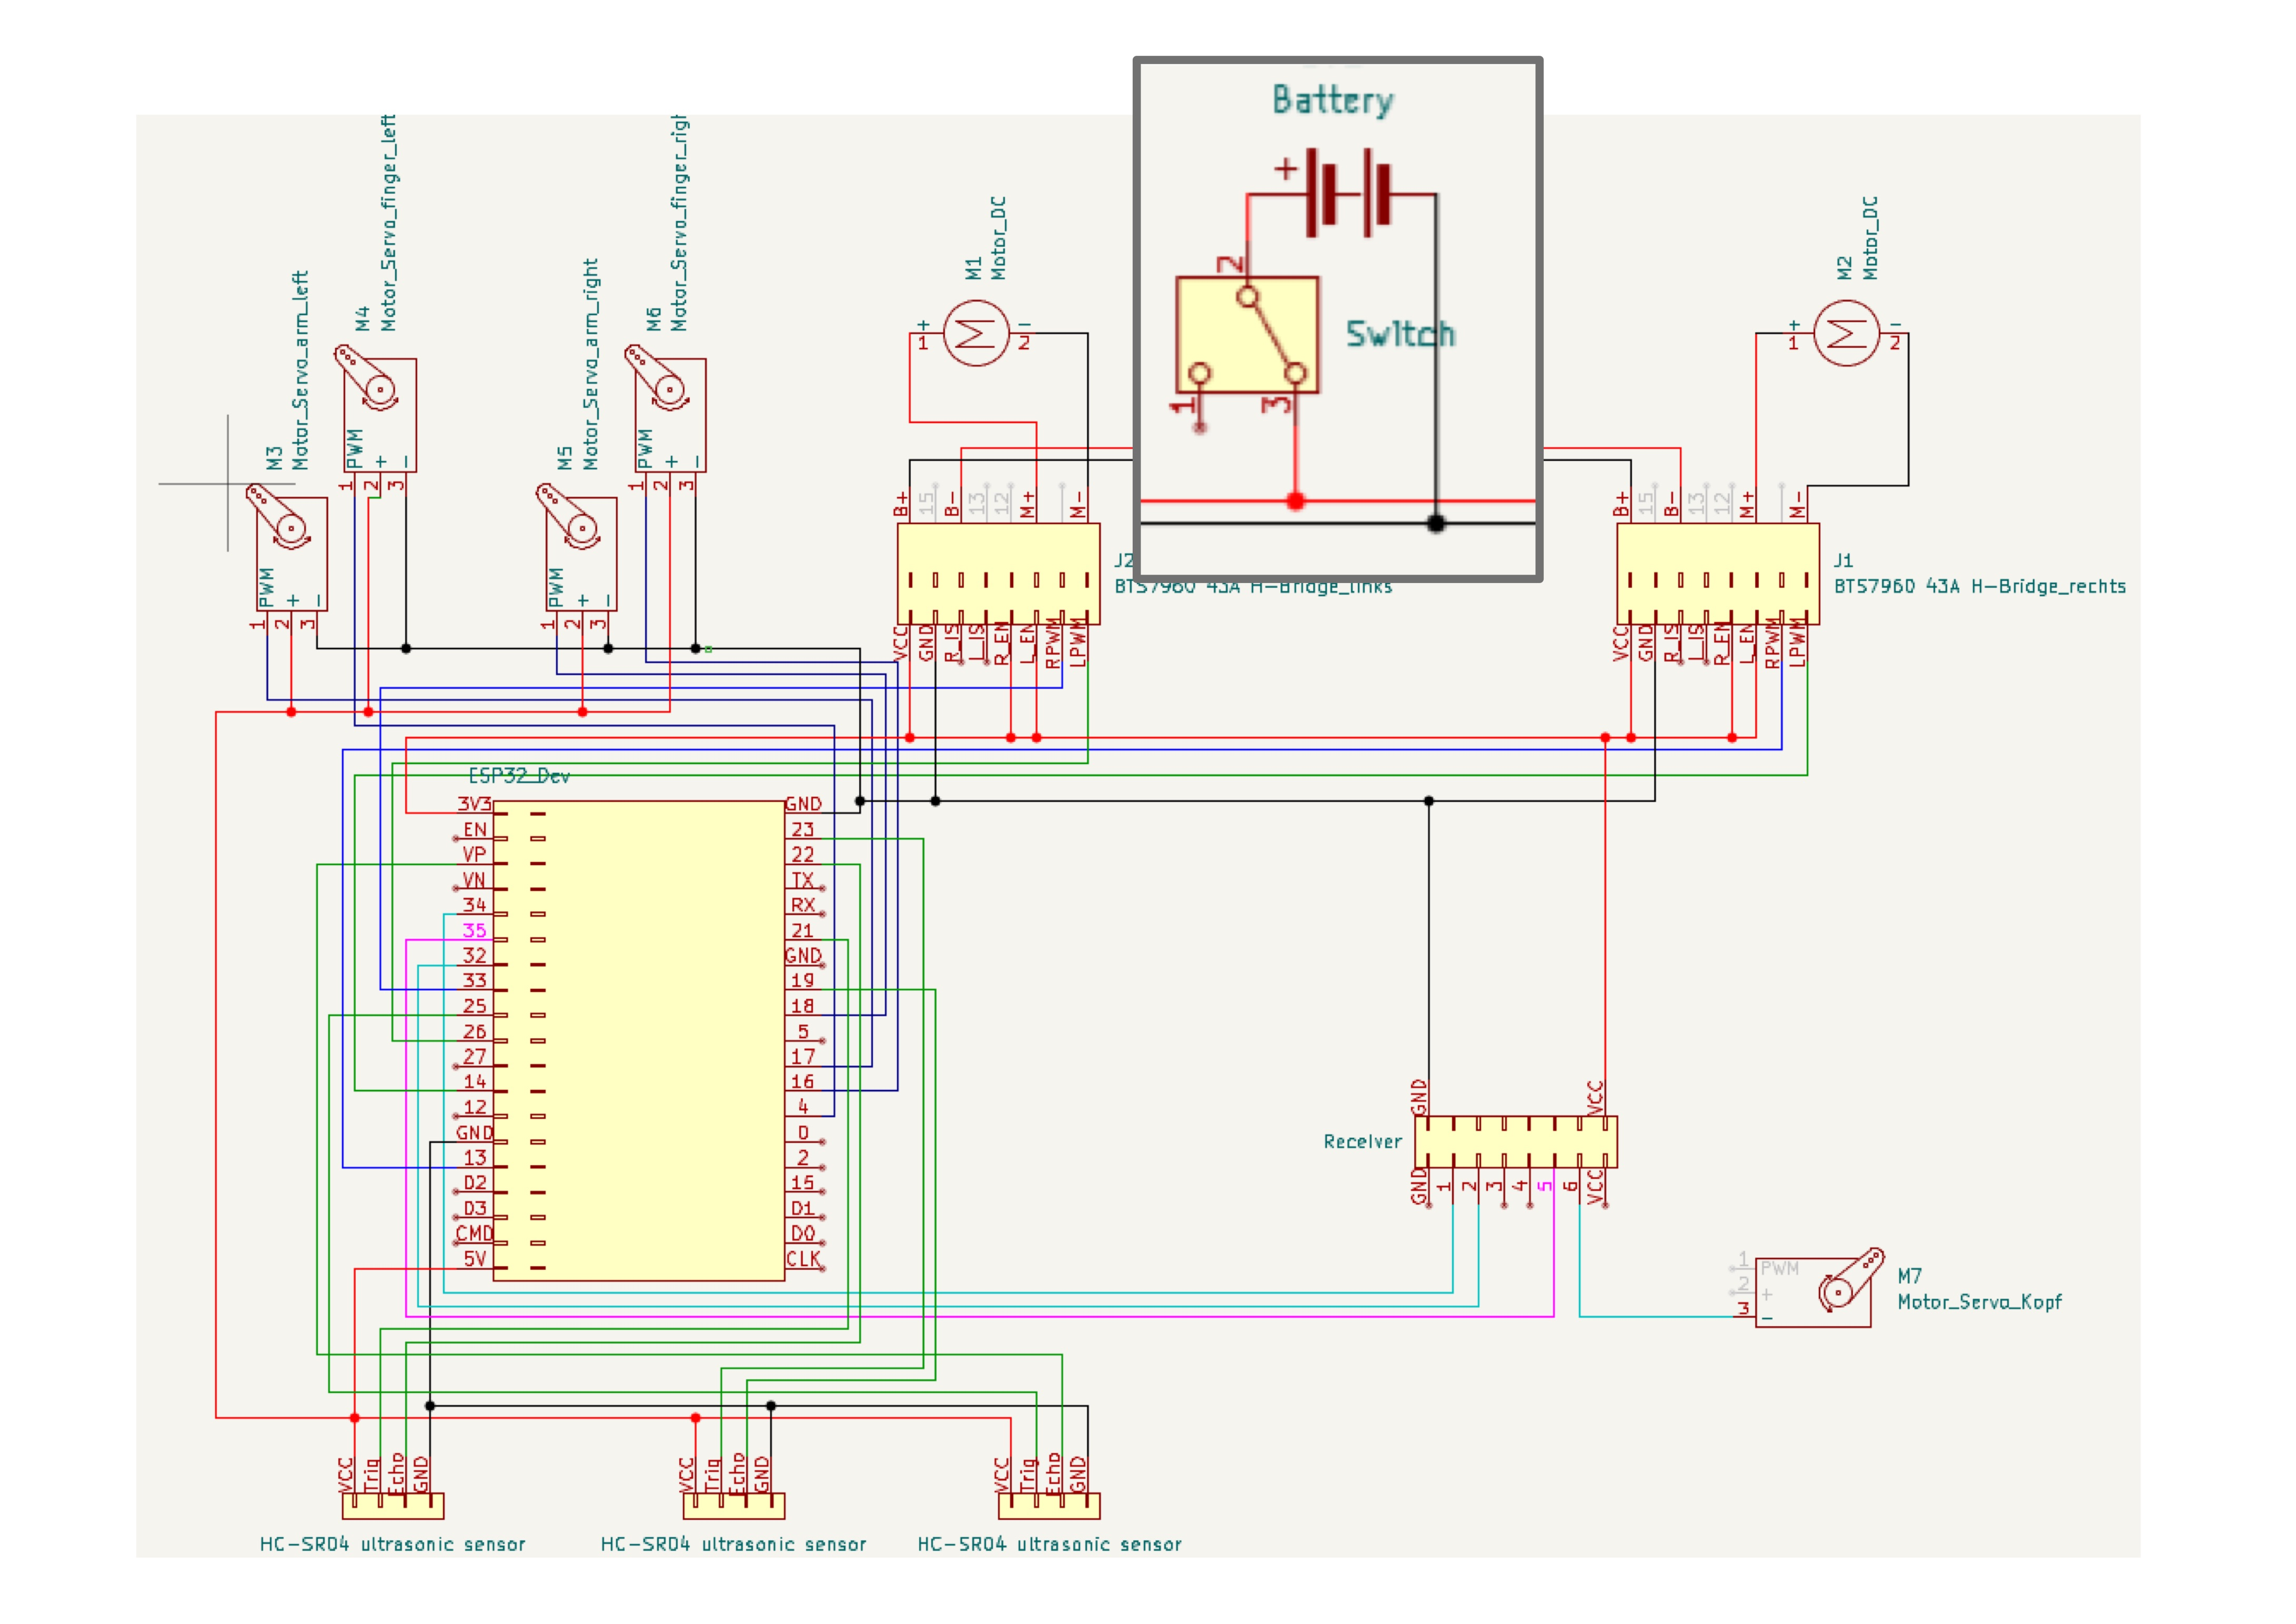
\includegraphics[width=1.1\linewidth]{images/schaltergross.png}
	\caption{Position des Notschalters im Schaltplan: Der Schalter ist
		zwischen Batterie und den H-Brücken der beiden Antriebsmotoren
		verbaut und unterbricht im Notfall die gesamte Stromversorgung der
		Motoren.}
	\label{fig:notschalterposition2}
\end{figure}